\section{Applications of Elliptic Partial Differential Equations}
\label{sec:applications}

We will look at two examples where the use of a fast elliptic PDE solver would greatly benefit the solution process. These are cases where an elliptic solve is required multiple times, such as every time step or for multiple problems.

\subsection{Navier-Stokes: The Projection Method}

The incompressible Navier-Stokes equations is a nonlinear PDE that arises from conservation of momentum and mass in an incompressible fluid. They are expressed as
\begin{align}
    \frac{\partial \textbf{u}}{\partial t} + \textbf{u} \cdot \nabla \textbf{u} &= -\frac{1}{\rho} \nabla P + \nu \nabla^2 \textbf{u}.
\end{align}
In \cite{chorin1967numerical}, Chorin first computes an intermediate velocity $\textbf{u}^*$ by time stepping and ignoring the pressure term
\begin{align}
    \frac{\textbf{u}^* - \textbf{u}^n}{\Delta t} &= -\textbf{u}^n \cdot \nabla \textbf{u}^n + \nu \nabla^2 \textbf{u}^n
\end{align}
and then ``projecting" the intermediate velocity to the next time step via
\begin{align}
    \textbf{u}^{n+1} = \textbf{u}^* - \frac{\Delta t}{\rho} \nabla P^{n+1}
\end{align}
In order to solve for the right-hand side of the second step, the pressure field at the $n+1$ time step must be known. This is found by solving the following Poisson's equation arising from taking the divergence of the second step and using the conservation of mass to eliminate the $\nabla \cdot \textbf{u}^{n+1}$ term:
\begin{align}
    \nabla^2 P^{n+1} &= \frac{\rho}{\Delta t} \nabla \cdot \textbf{u}^*
\end{align}

This projection method requires an elliptic solve at every time step to solve for the pressure field. In applications like this where an elliptic solve is required multiple times, direct methods where one can pre-compute the solution operator and then apply it each time step greatly speeds up the computation.

\subsection{The Shallow Water Equations and the Serre-Green-Naghdi Model}

\begin{figure}
    \centering
    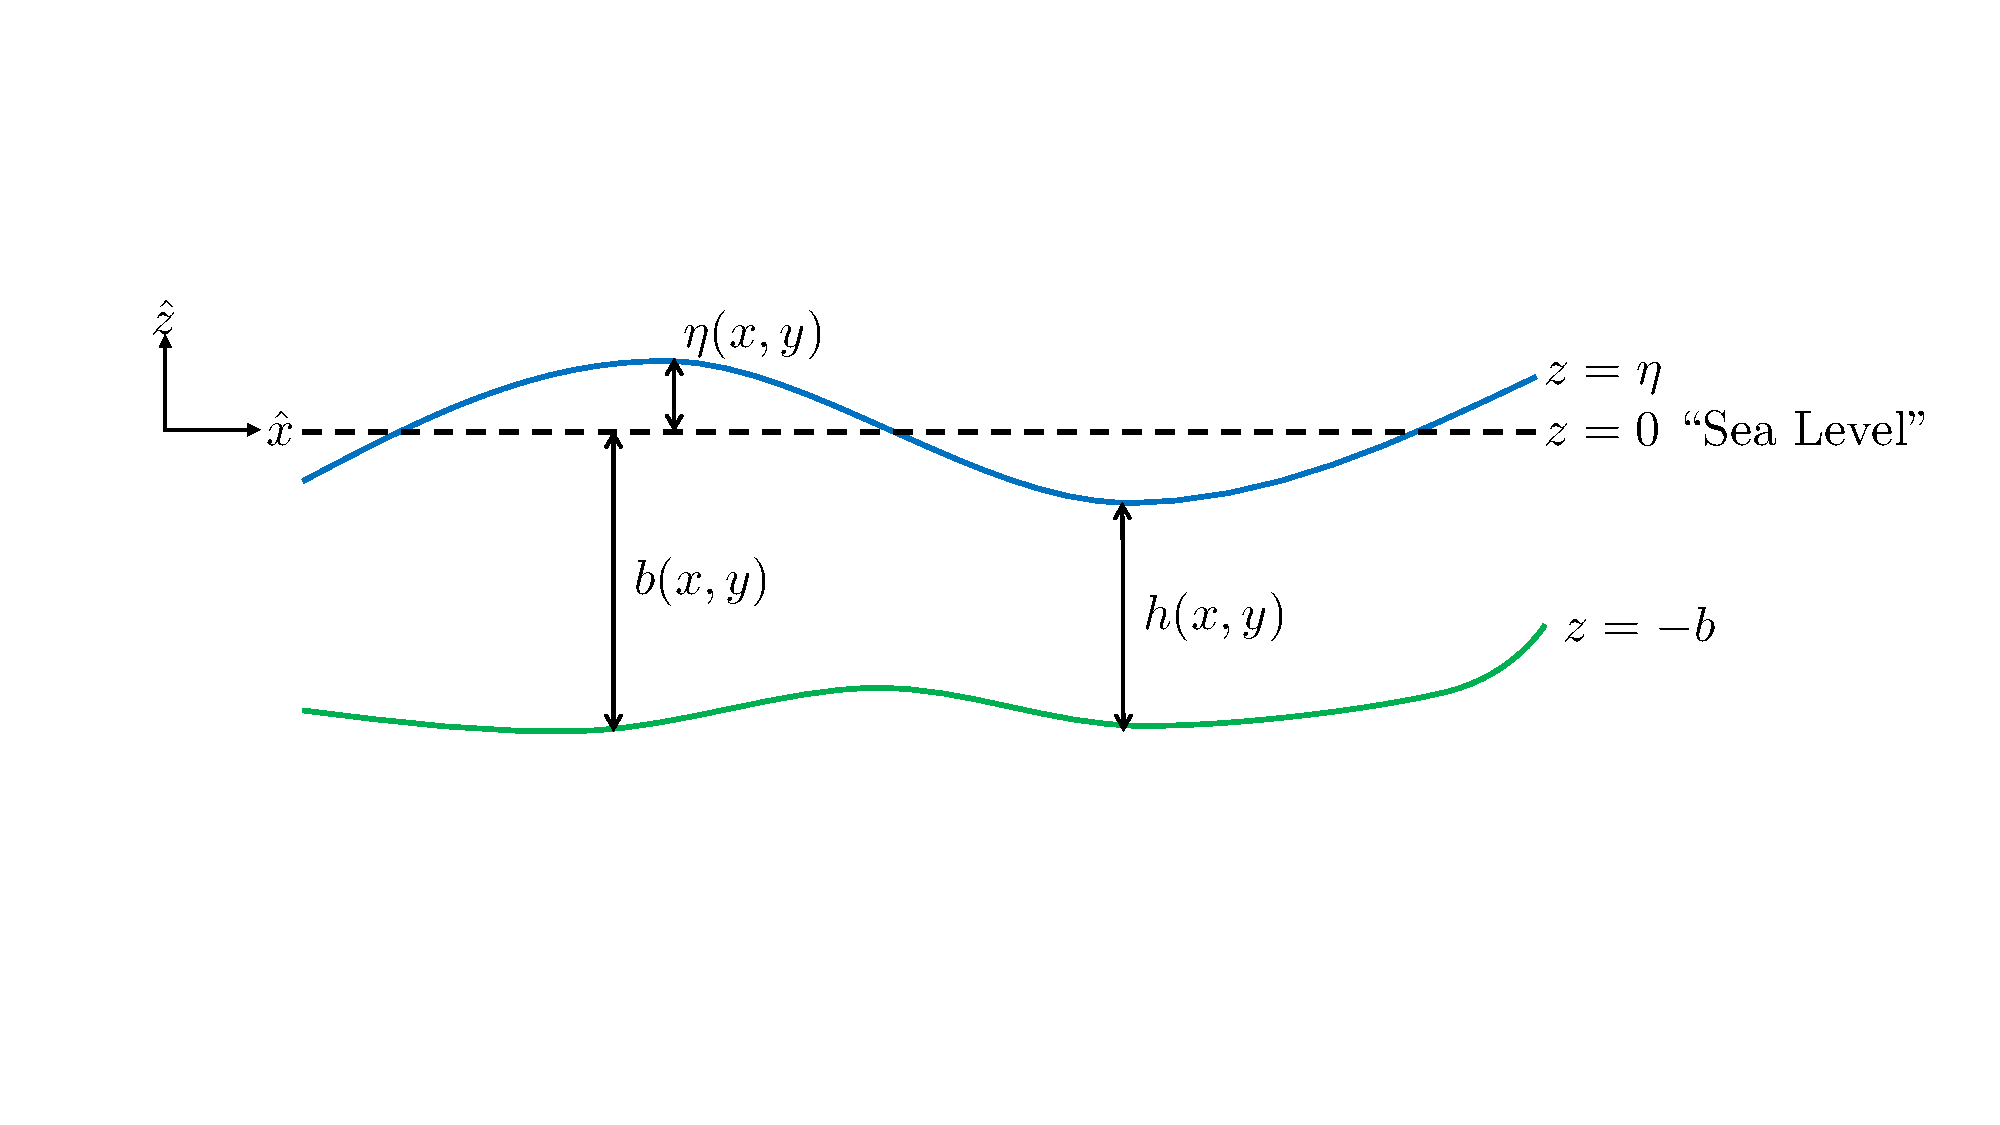
\includegraphics[width=\columnwidth]{../figures/swe_model.pdf}
    \caption{Shallow Water Equation Reference}
    \label{fig:swe}
\end{figure}

The shallow water equations (SWE) form a model for free surface flow derived from potential theory. The key assumption in the SWEs is that the horizontal scale is much larger than the vertical scale. Because a ``shallow limit" is assumed, the velocity field in the vertical direction is a depth-averaged velocity. These types of equations are used to model tsunami waves and debris flow, among other things.

Extensions to this model done by Bonneton et al. in \cite{bonneton2011splitting}, \cite{lannes2009derivation}, and \cite{lannes2015new} introduce a dispersive term correction in the form of a source term, leading to
\begin{align}
    \frac{\partial \textbf{q}}{\partial t} + \nabla \cdot \textbf{F}(\textbf{q}) = \textbf{b} + \textbf{s}
\end{align}
where
\begin{align}
    \textbf{q} &=
    \begin{bmatrix}
        h \\
        h u \\
        h v \\
    \end{bmatrix} \\
    \textbf{F}(\textbf{q}) &=
    \begin{bmatrix}
        h u & h v \\
        h u^2 + \frac{1}{2} gh^2 & h u v \\
        h u v & h v^2 + \frac{1}{2} gh^2 \\
    \end{bmatrix} \\
    \textbf{b} &=
    \begin{bmatrix}
        0 \\
        -g h \frac{\partial b}{\partial x} \\
        -g h \frac{\partial b}{\partial y} \\
    \end{bmatrix} \\
    \textbf{s} &=
    \begin{bmatrix}
        0 \\
        \frac{\alpha - 1}{\alpha} g h \frac{\partial \eta}{\partial x} + d_x \\
        \frac{\alpha - 1}{\alpha} g h \frac{\partial \eta}{\partial y} + d_y \\
    \end{bmatrix}.
\end{align}
The water column height is denoted by $h(x,y)$, with surface velocity $(u(x,y), v(x,y))$, $b(x,y)$ is a bathymetry term (elevation), $\eta(x,y)$ is the free surface height and dispersive term correction $(d_x, d_y)$. Figure \ref{fig:swe} shows the typical setup for this kind of problem.

In order to solve for the dispersive source term, one must solve the following elliptic equation
\begin{align}
    \big( \textbf{I} + \alpha \textbf{T}_{diag}^b \big) \textbf{d} = \textbf{f}(h, \textbf{u}, b, \eta)
\end{align}
where the details of the right-hand side function can be found in \cite{lannes2015new}. The operator $\textbf{T}_{diag}^b$ is an elliptic-like operator that does not change with time. So, for a static mesh, the dispersive operator can be factorized via a direct method and applied at each time step. This reduces the need to solve the elliptic PDE every time step to just an application of the solution operator every time step. If the mesh is adapted, the solution operator would need to be reformed. However, direct methods like the HPS method can allow for a local adjustment to the solution operator, further accelerating the solution.
